% meta.concepts: centroid by integration
% acknowledge: inspired by problem 5.36 of Beer, Johnston, and Mazurek (12th Edition)

\noindent Use direct integration to find the centroid of the area shown in terms of a and h.  


\begin{figure}[ht!]
  \centering
  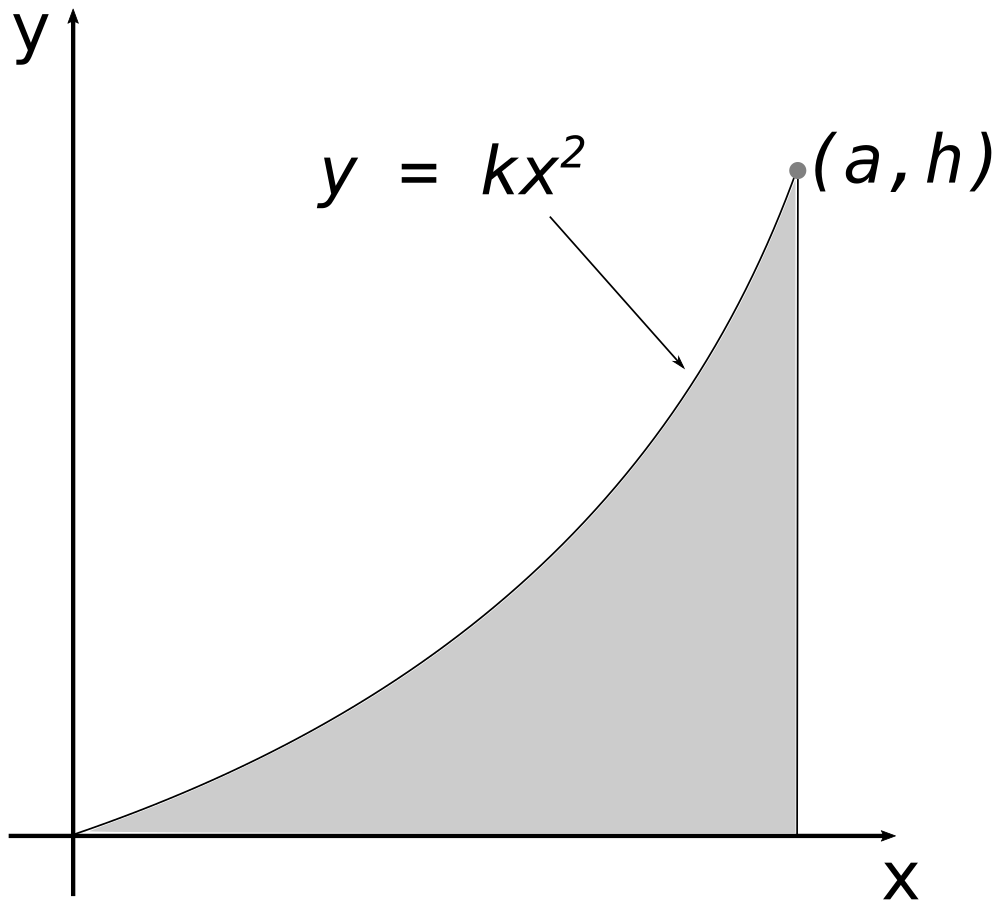
\includegraphics[height=1.8in]{fig.png}
\end{figure}


\iftoggle{flagSoln}{%
\vspace{.5cm}
\rule{\textwidth}{.4pt}
\vspace{.5cm}
\textbf{Solution:} 

Look up prabolic spandrel in the \textit{centroid of common shapes} figure/table (12th ed: Fig. 5.8A (12ed).
}{%
}%
